\documentclass[12pt]{article}
    % ------------------------------------------------------------------------
% PAKIETY
% ------------------------------------------------------------------------

%różne pakiety matematyczne, warto przejrzeć dokumentację, muszą być powyżej ustawień językowych.
\usepackage{mathrsfs}   %Różne symbole matematyczne opisane w katalogu ~\doc\latex\comprehensive. Zamienia \mathcal{L} ze zwykłego L na L-transformatę.
\usepackage{eucal}      %Różne symbole matematyczne.
\usepackage{amssymb}    %Różne symbole matematyczne.
\usepackage{amsmath}    %Dodatkowe funkcje matematyczne, np. polecenie \dfac{}{} skladajace ulamek w trybie wystawionym (porównaj $\dfrac{1}{2}$, a $\frac{1}{2}$).

\usepackage{tabularx} % tabela 100% width

%język polski i klawiatura
\usepackage[utf8]{inputenc} 
\usepackage[polish]{babel}
\usepackage[MeX]{polski}   %Strona kodowa polskich znaków.

%obsługa pdf'a
\usepackage[pdftex,usenames,dvipsnames]{color}      %Obsługa kolorów. Opcje usenames i dvipsnames wprowadzają dodatkowe nazwy kolorow.
\usepackage[pdftex,pagebackref=false,draft=false,pdfpagelabels=false,colorlinks=true,urlcolor=blue,linkcolor=red,citecolor=green,pdfstartview=FitH,pdfstartpage=1,pdfpagemode=UseOutlines,bookmarks=true,bookmarksopen=true,bookmarksopenlevel=2,bookmarksnumbered=true,pdfauthor={Marcin Szewczyk},pdftitle={Doktorat},pdfsubject={Praca doktorska},pdfkeywords={transient recovery voltage trv},unicode=true]{hyperref}   %Opcja pagebackref=true dotyczy bibliografii: pokazuje w spisie literatury numery stron, na których odwołano się do danej pozycji.

%bibliografia
\usepackage[numbers,sort&compress]{natbib}  %Porządkuje zawartość odnośników do literatury, np. [2-4,6]. Musi być pod pdf'em, a styl bibliogfafii musi mieć nazwę z dodatkiem 'nat', np. \bibliographystyle{unsrtnat} (w kolejności cytowania).
%\usepackage{hypernat}                       %Potrzebna pakietowi natbib do wspolpracy z pakietem hyperref (wazna kolejnosc: 1. hyperref, 2. natbib, 3. hypernat).

%grafika i geometria strony
\usepackage{extsizes}           %Dostepne inne rozmiary czcionek, np. 14 w poleceniu: \documentclass[14pt]{article}.
\usepackage[final]{graphicx}
\usepackage[a4paper,left=3.5cm,right=2.5cm,top=2.5cm,bottom=2.5cm]{geometry}

%strona tytułowa
\usepackage{strona_tytulowa}

%inne
\usepackage[hide]{todo}                     %Wprowadza polecenie \todo{treść}. Opcje pakietu: hide/show. Polecenie \todos ma byc na koncu dokumentu, wszystkie \todo{} po \todos sa ignorowane.
\usepackage[basic,physics]{circ}            %Wprowadza środowisko circuit do rysowania obwodów elektrycznych. Musi byc poniżej pakietow językowych.
\usepackage[sf,bf,outermarks]{titlesec}     %Troszczy się o wygląd tytułów rozdziałów (section, subsection, ...). sf oznacza czcionkę sans serif (typu arial), bf -- bold. U mnie: oddzielna linia dla naglowku paragraph. Patrz tez: tocloft -- lepiej robi format spisu tresci.
\usepackage{tocloft}                        %Troszczy się o format spisu trsci.
\usepackage{expdlist}    %Zmienia definicję środowiska description, daje większe możliwości wpływu na wygląd listy.
\usepackage{flafter}     %Wprowadza parametr [tb] do polecenia \suppressfloats[t] (polecenie to powoduje nie umieszczanie rysunkow, tabel itp. na stronach, na ktorych jest to polecenie (np. moze byc to stroma z tytulem rozdzialu, ktory chcemy zeby byl u samej gory, a nie np. pod rysunkiem)).
\usepackage{array}       %Ładniej drukuje tabelki (np. daje wiecej miejsca w komorkach -- nie są tak ścieśnione, jak bez tego pakietu).
\usepackage{listings}    %Listingi programow.
\usepackage[format=hang,labelsep=period,labelfont={bf,small},textfont=small]{caption}   %Formatuje podpisy pod rysunkami i tabelami. Parametr 'hang' powoduje wcięcie kolejnych linii podpisu na szerokosc nazwy podpisu, np. 'Rysunek 1.'.
\usepackage{appendix}    %Troszczy się o załączniki.
\usepackage{floatflt}    %Troszczy się o oblewanie rysunkow tekstem.
\usepackage{here}        %Wprowadza dodtkowy parametr umiejscowienia rysunków, tabel, itp.: H (duże). Umiejscawia obiekty ruchome dokladnie tam gdzie są w kodzie źródłowym dokumentu.
\usepackage{makeidx}     %Troszczy się o indeks (skorowidz).


%nieużywane, ale potencjalnie przydatne
%\usepackage{sectsty}           %Formatuje nagłówki, np. żeby były kolorowe -- polecenie: \allsectionsfont{\color{Blue}}.
%\usepackage{version}           %Wersje dokumentu.
%\usepackage{fancyhdr}          %Dodaje naglowki jakie się chce.
%\usepackage{antyktor}          %Składa dokument przy użyciu Antykwy Toruńskiej.
%\usepackage{antpolt}           %Składa dokument przy użyciu Antykwy Półtawskiego.
%\usepackage[left]{showlabels}  %Pokazuje etykiety, ale kiepsko bo nie mieszcza sie na marginesie (można od biedy powiększyć margines w pakiecie geometry powyżej). Nie może być na górze (pakiet).

    % ------------------------------------------------------------------------
% USTAWIENIA
% ------------------------------------------------------------------------

% ------------------------------------------------------------------------
%   Kropki po numerach sekcji, podsekcji, itd.
%   Np. 1.2. Tytuł podrozdziału
% ------------------------------------------------------------------------
\makeatletter
    \def\numberline#1{\hb@xt@\@tempdima{#1.\hfil}}                      %kropki w spisie treści
    \renewcommand*\@seccntformat[1]{\csname the#1\endcsname.\enspace}   %kropki w treści dokumentu
\makeatother

% ------------------------------------------------------------------------
%   Numeracja równań, rysunków i tabel
%   Np.: (1.2), gdzie:
%   1 - numer sekcji, 2 - numer równania, rysunku, tabeli
%   Uwaga ogólna: o otoczeniu figure ma być najpierw \caption{}, potem \label{}, inaczej odnośnik nie działa!
% ------------------------------------------------------------------------
\makeatletter
    \@addtoreset{equation}{section} %resetuje licznik po rozpoczęciu nowej sekcji
    \renewcommand{\theequation}{{\thesection}.\@arabic\c@equation} %dodaje kropkę

    \@addtoreset{figure}{section}
    \renewcommand{\thefigure}{{\thesection}.\@arabic\c@figure}

    \@addtoreset{table}{section}
    \renewcommand{\thetable}{{\thesection}.\@arabic\c@table}
\makeatother

% ------------------------------------------------------------------------
% Tablica
% ------------------------------------------------------------------------
\newenvironment{tablica}[3]
{
    \begin{table}[!tb]
    \centering
    \caption[#1]{#2}
    \vskip 9pt
    #3
}{
    \end{table}
}

% ------------------------------------------------------------------------
% Dostosowanie wyglądu pozycji listy \todos, np. zamiast 'p.' jest 'str.'
% ------------------------------------------------------------------------
\renewcommand{\todoitem}[2]{%
    \item \label{todo:\thetodo}%
    \ifx#1\todomark%
        \else\textbf{#1 }%
    \fi%
    (str.~\pageref{todopage:\thetodo})\ #2}
\renewcommand{\todoname}{Do zrobienia...}
\renewcommand{\todomark}{~uzupełnić}

% ------------------------------------------------------------------------
% Definicje
% ------------------------------------------------------------------------
\def\nonumsection#1{%
    \section*{#1}%
    \addcontentsline{toc}{section}{#1}%
    }
\def\nonumsubsection#1{%
    \subsection*{#1}%
    \addcontentsline{toc}{subsection}{#1}%
    }
\reversemarginpar %umieszcza notki po lewej stronie, czyli tam gdzie jest więcej miejsca
\def\notka#1{%
    \marginpar{\footnotesize{#1}}%
    }
\def\mathcal#1{%
    \mathscr{#1}%
    }
\newcommand{\atp}{ATP/EMTP} % Inaczej: \def\atp{ATP/EMTP}

% ------------------------------------------------------------------------
% Inne
% ------------------------------------------------------------------------
\frenchspacing                      %nie pamiętam co to jest, ale używam
%\flushbottom                       %nie pamiętam co to jest, ale nie używam
%\raggedbottom                      %nie pamiętam co to jest, ale nie używam
\hyphenation{ATP/-EMTP}             %dzielenie wyrazu w żądanym miejscu
\setlength{\parskip}{3pt}           %odstęp pomiędzy akapitami
\linespread{1.2}                    %odstęp pomiędzy liniami (interlinia)
\setcounter{tocdepth}{4}            %uwzględnianie w spisie treści czterech poziomów sekcji
\setcounter{secnumdepth}{4}         %numerowanie do czwartego poziomu sekcji włącznie
\titleformat{\paragraph}[hang]      %wygląd nagłówków
{\normalfont\sffamily\bfseries}{\theparagraph}{1em}{}
%\definecolor{niebieski}{rgb}{0.0,0.0,0.5}

    % !TEX program = pdflatex
    \title{Projekt sieci komputerowej \\ oraz instalacji elektrycznej budynku.}
    \author{\\Piotr Błądek \\Piotr Gołaszewski}

    %polecenia zdefiniowane w pakiecie strona_tytulowa.sty
    \uczelnia{POLITECHNIKA WARSZAWSKA}
    \instytut{Instytut Elektroenergetyki \\  Politechniki Warszawskiej}
    \promotor{dr hab inż. Pawła Piotrowskiego}
    \praca{Projekt}
    \rok{2015}
    %\draft  %odkomentarzuj tę linię, jeśli wydruk ma być draftem -- wprowadza informację o drafcie na stronie tytułowej
    %koniec poleceń zdefiniowanych przez pakiet strona_tytulowa.sty

    %skorowidz - nie używam
    %\makeindex
    %koniec skorowidza

\begin{document}
    \renewcommand{\figurename}{Rys.}    %musi byc pod \begin{document}, bo w~tym miejscu pakiet 'babel' narzuca swoje ustawienia
    \renewcommand{\tablename}{Tab.}     %j.w.
    %\pagenumbering{roman}               %numeracja stron: rzymska
    \thispagestyle{empty}               %na tej stronie: brak numeru
    \stronatytulowa                     %strona tytułowa tworzona przez pakiet strona_tytulowa.tex

    %podziękowania
    %\newpage
    %~   %potrzebne dla \vfill
    %\vfill
    %{\sffamily
    %\begin{flushright}
      %  \begin{tabular}{l}
       % Chciałbym w~tym miejscu podziękować:\\
       % \\
       % Kolegom i koleżankom z Klubu\\
        %-- za udane wakacje, które przyczyniły się\\
        %do powstania tej pracy\\
        %\\
        %Bosmanowi ze Sztynortu\\
        %-- za naprawienie silnika, itp.\\
        %\end{tabular}
    %\end{flushright}
    %}
    %\vskip0.5in
    %\thispagestyle{empty}
    
    
    
    %\newpage
    %koniec podziękowań

    %formatowanie spisu treści i~nagłówków
    \renewcommand{\cftbeforesecskip}{8pt}
    \renewcommand{\cftsecafterpnum}{\vskip 8pt}
    \renewcommand{\cftparskip}{3pt}
    \renewcommand{\cfttoctitlefont}{\Large\bfseries\sffamily}
    \renewcommand{\cftsecfont}{\bfseries\sffamily}
    \renewcommand{\cftsubsecfont}{\sffamily}
    \renewcommand{\cftsubsubsecfont}{\sffamily}
    \renewcommand{\cftparafont}{\sffamily}
    %koniec formatowania spisu treści i nagłówków

    \tableofcontents    %spis treści
    %\newpage

    %\input{wykaz_skrotow.tex}
    %\newpage

    %spis rysunków i~tablic
    %format spisu treści dotyczy tylko tych spisów, które są poniżej
    \hypersetup{linkcolor=black}
    \renewcommand{\cftparskip}{3pt}
    \renewcommand{\cftloftitlefont}{\Large\bfseries\sffamily}
    \listoffigures
    \addcontentsline{toc}{section}{Spis rysunków}
    %\addcontentsline{toc}{section}{Spis tablic}
    \newpage
    %powrót do czerwonego koloru dla dalszych odnośników (spis literatury, przy włączonym pokazywaniu numerów stron, do których odnoszą się poszczególne pozycje)
    \hypersetup{linkcolor=black}
    %koniec spisu rysunków i~tablic

    %przeniesienie wartości licznika stron na strony numerowane innym stylem (arabic)
    \newcounter{licznikStron}
    \setcounter{licznikStron}{\value{page}}
    \pagenumbering{arabic}
    \setcounter{page}{\value{licznikStron}}
    %koniec przeniesienia...

    %treść główna dokumentu
    \section{Przykładowa lista}
\suppressfloats[t]
\begin{itemize}
  \item \textit{yyy} - ola ma psa
  \item \textit{zzz} - ela ma misia
  \item \textit{xxx} - ala ma kota
\end{itemize}



\section{Przykładowa tabela}

\begin{tabularx}{\textwidth}{X|l|X}
\hline
\textbf{A} & \textbf{B} & \textbf{Ce} \\ \hline
xxx         & xxx         & xxx          \\ \hline
yyy          &yyy         & yyy            \\ \hline
\end{tabularx}

\section{Przykładowy rysunek}

\begin{figure}[!tb]
    \centering
    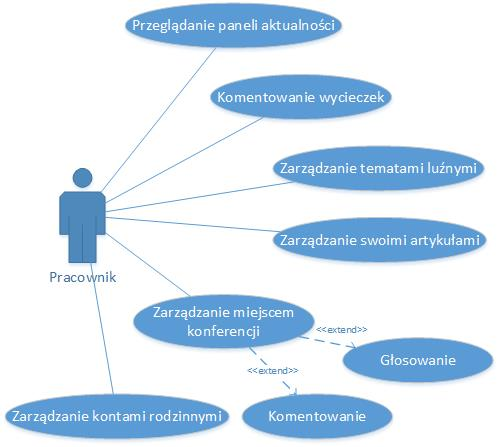
\includegraphics{pracownik.jpg}
    \caption{Przykładowy rysunek.}
    \label{fig:pracownik}
\end{figure}

\section{}
    \newpage
    %koniec treści głównej dokumentu

    %bibliografia
    %GATHER{bibliografia.bib}                       %polecenie programu WinEdt, włącza plik do drzewa 'projektu'
    %\bibliographystyle{unsrtnat}                    %styl bibliografii: w kolejności cytowania, zrozumiały dla pakietu hyperref.sty
    %\addcontentsline{toc}{section}{Literatura}      %musi być wyżej niż \bibliography{bibliografia}, żeby w~spisie treści był właściwy numer strony
    %\bibliography{bibliografia}
    %koniec bibliografii

    %załączniki
    %\newpage
    %\appendix
    %\renewcommand{\appendixtocname}{Załączniki}
    %\renewcommand{\appendixpagename}{~\vspace{8cm} \begin{center}Załączniki\end{center}\newpage}
    %\thispagestyle{empty}
    %\addappheadtotoc
    %\appendixpage
    %\input{zalacznik.tex}
    %koniec załączników

    %skorowidz - nie używam
%    \index{Napis}
%    \index{Napis!Podnapis}
%    \printindex
    %koniec skorowidza

    %lista rzeczy do zrobienia: wypisuje na końcu dokumentu, patrz: pakiet todo.sty
    \todos
    %koniec listy rzeczy do zrobienia
\end{document}
